\documentclass[a4paper,onecolumn,pdftex]{report}

\usepackage{graphicx}
\usepackage{wrapfig}
\usepackage[p,osf]{scholax}
\usepackage{amsmath}
\usepackage{MnSymbol}
\usepackage[scaled=1.075,ncf,vvarbb]{newtxmath}
\usepackage[margin=1in]{geometry}

\fontfamily{scholax}
\overfullrule=0pt

\begin{document}
    \author{Noah Tjorven Burdorf}
    \title{Mitschrieb \\ Mathematik 1 \\ Vorlesung vom 10.10.2023}
    \date{10.10.2023}
    \maketitle

    \section*{1 - zu Seite 33}
    \subsection*{Infos vorraus}
    \begin{wrapfigure}[3]{l}{.5\textwidth}
        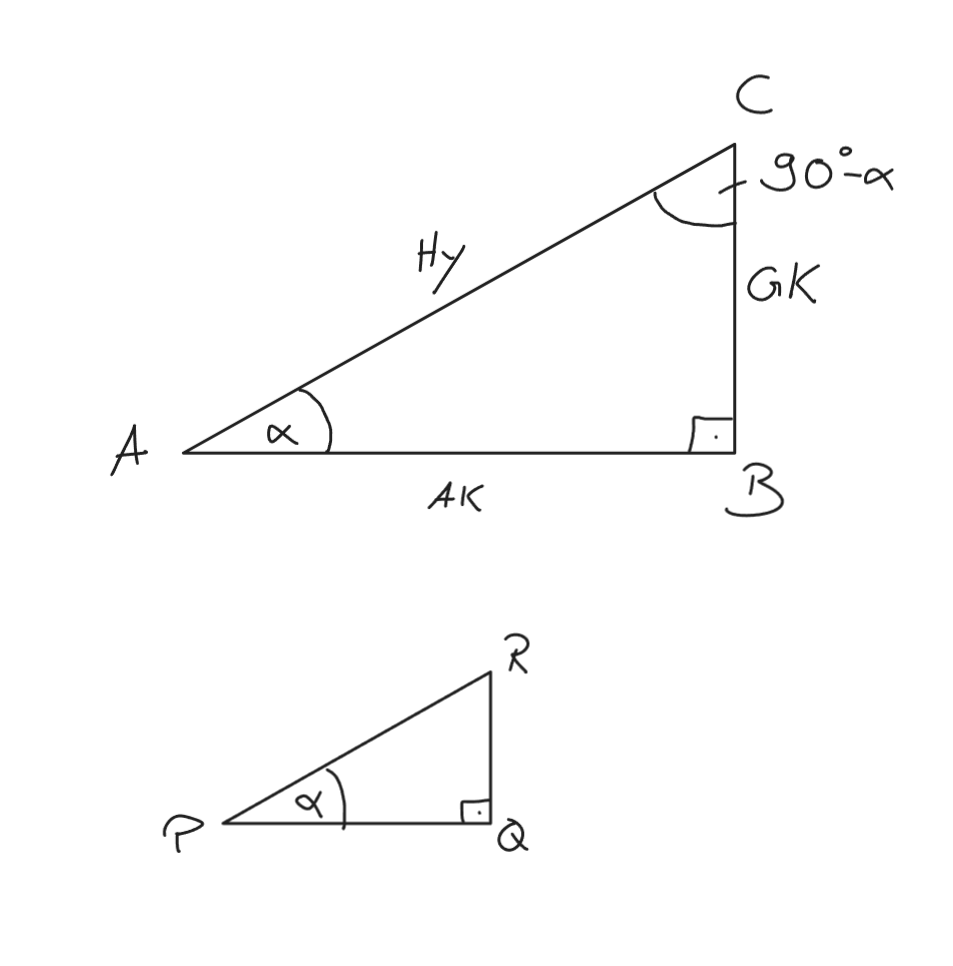
\includegraphics[width=6cm]{2023-10-10_22h01_07.png}
    \end{wrapfigure}
    AC $\hateq$ Vector \\
    |AC| $\hateq$ Stecke \\
    ||AC|| $\hateq$ L\"ange \\
    \begin{align*}
        \sin\alpha&=\frac{Gk}{Hy}=\frac{||BC||}{||AC||}=\frac{||CB||}{||CA||} \\
        \cos\alpha&=\frac{Ak}{Hy}=\frac{||AB||}{||AC||} \\
        \tan\alpha&=\frac{Gk}{Ak} \\\\
        \sin(90-\alpha) = \frac{||AB||}{||AC||} = \cos\alpha
    \end{align*}
    \subsection*{Zwei Dreiecke sind \"ahnlich wenn deren Winkel gleich gross sind.}
    $$\Delta ABC \backsim \Delta PQR \Rightarrow \frac{||AC||}{||PR||}=\frac{||BC||}{||QR||}=\frac{||AB||}{||PQ||}$$
    SATZ DES THALES!!!
    \subsection*{Positionen und Gradmass zu Bogenmass}
    \begin{wrapfigure}{l}{0.3\textwidth}
        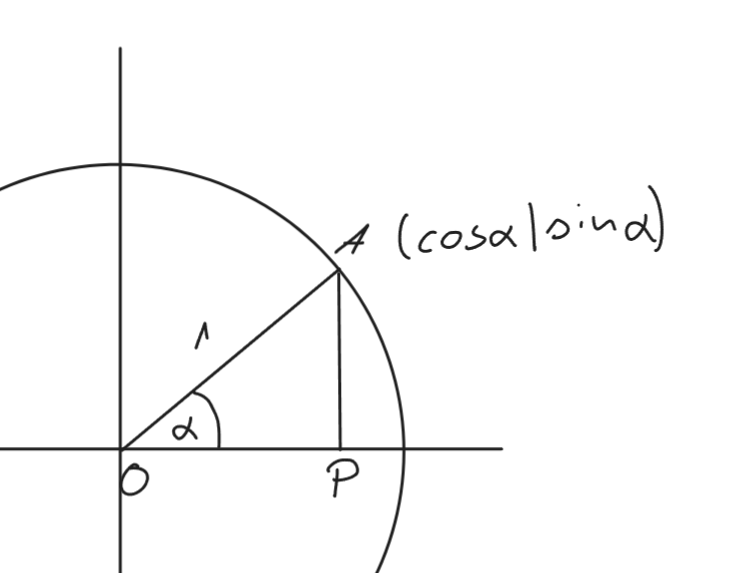
\includegraphics[width=6cm]{2023-10-10_21h42_30.png}
    \end{wrapfigure}
    \begin{align*}
        360^\circ &\hateq 2\pi \\
        180^\circ &\hateq \pi \\
        90^\circ &\hateq \frac{\pi}{2} \\
        60^\circ &\hateq \frac{\pi}{3} \\
        45^\circ &\hateq \frac{\pi}{4} \\
        30^\circ &\hateq \frac{\pi}{6} \\
        \cos(-\alpha) &= \cos\alpha \\
        \sin(-\alpha) &= -\sin\alpha \\
        \sin(90-\alpha) &= cos\alpha \\
        \cos(90-\alpha) &= \sin\alpha \\
        \sin^2\alpha + \cos^2\alpha &= 1
    \end{align*}


\end{document}